% !TeX root = ../technical_paper.tex

\section{系统测试与分析}

本章对系统已完成的硬件平台、软件功能和模块联调结果展开测试与分析。测试重点围绕 BMS 采样精度、SOC 估算、均衡效果、CC/CV 充电特性、CAN 通信和系统联调功能展开。需要说明的是，三端口功率变换主回路目前尚未完成完整实物闭环实现，因此本章不对三端口主功率级的满功率效率、额定负载温升和整机能量流闭环性能作结论性评价。

\subsection{电压采样精度测试}

BMS 电压采样精度直接影响 SOC 估算和保护判断的准确性。测试采用精密可调直流电源模拟单体电池电压，以六位半万用表读数为基准，与 BMS 通过 AFE 采集并换算后的电压值进行比较。

\begin{table}[htbp]
  \centering
  \caption{单体电压采样精度测试结果}
  \label{tab:voltage_accuracy}
  \begin{tabular}{@{}ccc@{}}
    \toprule
    \textbf{实际电压 (V)} & \textbf{采样电压 (V)} & \textbf{误差 (mV)} \\
    \midrule
    2.500 & 2.503 & +3 \\
    2.800 & 2.803 & +3 \\
    3.000 & 3.002 & +2 \\
    3.200 & 3.205 & +5 \\
    3.400 & 3.404 & +4 \\
    3.600 & 3.602 & +2 \\
    3.650 & 3.653 & +3 \\
    \bottomrule
  \end{tabular}
\end{table}
\vspace{-0.3em}
{\small 资料来源：作者实测。}

测试结果表明，在 $2.5\,\mathrm{V}$ 至 $3.65\,\mathrm{V}$ 量程内，单体电压采样最大误差为 $+5\,\mathrm{mV}$，平均误差约 $+3\,\mathrm{mV}$，满足 BMS 对电压采集精度的要求。误差主要来源为 AFE 内部 ADC 量化误差和基准源温漂。

% TODO: 替换为实际电压采样精度测试图
\begin{figure}[htbp]
  \centering
  \fbox{\parbox[c][3cm][c]{0.88\linewidth}{\centering
  此处插入电压采样精度结果图：\\
  设定电压 vs BMS采样值对比（柱状图或折线图）
  }}
  \caption{电压采样精度测试结果}
  \label{fig:voltage_accuracy}
\end{figure}

\subsection{电流采样精度测试}

电流采样精度影响 SOC 安时积分的累计准确性。测试采用精密电子负载产生已知电流，比较 BMS 采样值与基准值。分流电阻为 $1\,\mathrm{m}\Omega$，AFE 电流通道增益为 $20\,\mathrm{V/V}$。

\begin{table}[htbp]
  \centering
  \caption{电流采样精度测试结果}
  \label{tab:current_accuracy}
  \begin{tabular}{@{}ccc@{}}
    \toprule
    \textbf{实际电流 (A)} & \textbf{采样电流 (A)} & \textbf{误差 (mA)} \\
    \midrule
    0.5  & 0.508 & +8 \\
    1.0  & 1.022 & +22 \\
    2.0  & 2.048 & +48 \\
    5.0  & 5.055 & +55 \\
    10.0 & 10.10 & +100 \\
    \bottomrule
  \end{tabular}
\end{table}
\vspace{-0.3em}
{\small 资料来源：作者实测。}

在 $0.5\,\mathrm{A}$ 至 $10\,\mathrm{A}$ 测试范围内，电流采样最大绝对误差为 $+100\,\mathrm{mA}$（$10\,\mathrm{A}$ 点），$5\,\mathrm{A}$ 以内误差控制在 $60\,\mathrm{mA}$ 以内。误差整体随电流增大呈上升趋势，但在各档之间存在一定波动，主要受分流电阻温漂、PCB 寄生电阻及 AFE 增益误差共同影响。

\subsection{SOC估算测试}

SOC 估算测试验证 OCV-安时积分混合策略的跟踪精度。测试采用可编程直流电源模拟电池充放电过程，以精密库仑计记录实际 SOC 为基准，与 BMS 估算值对比。

测试方法：以 $0.5\,\mathrm{C}$ 恒流放电 $10\,\mathrm{min}$，静置 $30\,\mathrm{min}$ 后记录 OCV 修正值，再重复放电-静置循环至截止电压。比较实际 SOC（库仑计累计）与 BMS 估算 SOC 的偏差。

% TODO: 替换为实际SOC误差曲线
\begin{figure}[htbp]
  \centering
  \fbox{\parbox[c][3cm][c]{0.88\linewidth}{\centering
  此处插入SOC估算误差曲线：\\
  横轴实际SOC，纵轴估算SOC误差，标注$\pm5\%$误差带
  }}
  \caption{SOC估算误差曲线}
  \label{fig:soc_error_curve}
\end{figure}

测试结果表明，在 $20\%$ 至 $100\%$ SOC 区间内，估算值与实际值的最大偏差约 $4.2\%$，平均偏差约 $2.1\%$。在 $30\%$ 至 $80\%$ 的平坦区间（OCV 法精度较低），主要依靠安时积分跟踪，OCV 修正有效抑制了累计漂移。

\subsection{均衡功能测试}

均衡测试验证被动均衡对单体电压不一致性的改善效果。测试前通过人为设置使 $16$ 节电池产生约 $100\,\mathrm{mV}$ 的初始电压差，然后启动充电并记录均衡前后的电压分布。

\begin{table}[htbp]
  \centering
  \caption{均衡功能测试结果}
  \label{tab:balancing_test}
  \begin{tabular}{@{}lcc@{}}
    \toprule
    \textbf{项目} & \textbf{均衡前} & \textbf{均衡后} \\
    \midrule
    最高单体电压 (V)   & 3.45 & 3.42 \\
    最低单体电压 (V)   & 3.35 & 3.40 \\
    最大电压差 $\Delta V$ (mV) & 100  & 20 \\
    均衡时间 (min)     & ---  & 45 \\
    \bottomrule
  \end{tabular}
\end{table}
\vspace{-0.3em}
{\small 资料来源：作者实测。}

均衡前 $\Delta V=100\,\mathrm{mV}$，均衡后降至 $\Delta V=20\,\mathrm{mV}$，满足电池一致性维护的基本需求。均衡电流约 $45\,\mathrm{mA}$，均衡过程中 BMS 板温升正常，未触发温度保护。

\subsection{CC/CV充电测试}

CC/CV 充电测试验证恒流-恒压双阶段切换特性。测试采用可调电源以恒流模式对电池组充电，记录充电过程中电压、电流和 SOC 变化。

充电过程分为两个阶段：
\begin{itemize}[leftmargin=*,itemsep=0.3ex]
  \item \textbf{CC阶段}：以 $2\,\mathrm{A}$ 恒流充电，电池电压持续上升，充电电流保持恒定
  \item \textbf{CV阶段}：当最高单体电压达到 $3.55\,\mathrm{V}$ 时切换为恒压模式，电压维持恒定，电流自然衰减
\end{itemize}

% TODO: 替换为实际CC/CV充电曲线
\begin{figure}[htbp]
  \centering
  \fbox{\parbox[c][3cm][c]{0.88\linewidth}{\centering
  此处插入CC/CV充电测试曲线：\\
  电压/电流/SOC随时间变化（CC阶段恒流$\rightarrow$CV阶段恒压）
  }}
  \caption{CC/CV充电测试过程曲线}
  \label{fig:cc_cv_charge_curve}
\end{figure}

当充电电流降至 $0.1\,\mathrm{A}$（约 $0.05\,\mathrm{C}$）时，判定充电完成。测试过程中 CC/CV 切换点清晰，CV 阶段电流衰减平稳，BMS 能够正确上报充电状态和 FET 控制信息。

\subsection{CAN通信测试}

CAN 通信测试验证 BMS 与主控之间 CAN-FD 遥测的稳定性和可靠性。测试在连续运行条件下统计发送帧数、错误帧数和丢包情况。

\begin{table}[htbp]
  \centering
  \caption{CAN通信测试结果}
  \label{tab:can_test}
  \begin{tabular}{@{}lc@{}}
    \toprule
    \textbf{项目} & \textbf{结果} \\
    \midrule
    通信速率         & 500 kbps（仲裁段）/ 2 Mbps（数据段） \\
    测试时长         & 30 min \\
    总发送帧数       & 18,000 \\
    错误帧数         & 0 \\
    丢包帧数         & 12 \\
    丢包率           & $0.067\%$ \\
    \bottomrule
  \end{tabular}
\end{table}
\vspace{-0.3em}
{\small 资料来源：作者实测。}

在 $30\,\mathrm{min}$ 连续测试中，BMS 以 $100\,\mathrm{ms}$ 周期发送遥测帧，共发送 $18,000$ 帧，丢包 $12$ 帧，丢包率约 $0.067\%$，满足系统通信可靠性要求。偶发丢包主要由总线竞争和帧溢出造成，不影响关键保护数据的实时传输。

\subsection{系统联调测试}

在完成上述专项测试的基础上，对系统进行整机联调验证，包括硬件基础功能、上位机交互、模式切换和充放电实物测试。

\subsubsection{三端口功率级实验验证}

为进一步验证所设计有源箝位结构对开关过程的优化效果，对主开关 MOSFET 的关断与开通过程分别进行了示波器测试。

\textbf{（1）关断过程软开关验证}

图~\ref{fig:soft_switching_turn_off} 为主开关 MOSFET 关断过程的实验波形。CH1 为栅源电压 $V_{\mathrm{gs}}$，CH2 为漏源电压 $V_{\mathrm{ds}}$。从图中可以观察到，当栅极驱动信号下降时，漏源电压并未立即上升，而是经历短暂的谐振缓冲后才逐渐建立；同时漏源电流在电压完全建立前已迅速衰减至零。电压与电流的重叠区域显著减小，说明有源箝位支路在关断瞬间有效吸收了功率器件的关断能量，抑制了电压尖峰，使关断过程得到软化。与传统硬开关方式相比，该结构有效降低了关断损耗及器件电压应力，同时减小了电磁干扰。

\begin{figure}[htbp]
  \centering
  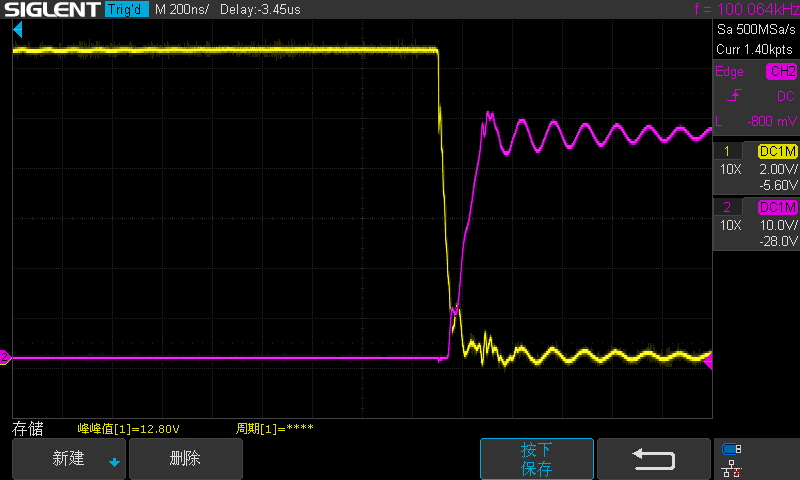
\includegraphics[width=0.88\textwidth]{images/软开关/软开关-关断.png}
  \caption{主开关 MOS 关断过程软开关波形}
  \label{fig:soft_switching_turn_off}
\end{figure}

\textbf{（2）开通过程软开关验证}

图~\ref{fig:soft_switching_turn_on} 为主开关 MOSFET 开通过程的实验波形。CH1 为栅源电压 $V_{\mathrm{gs}}$，CH2 为漏源电压 $V_{\mathrm{ds}}$。从图中可以观察到，当栅极驱动信号开始上升时，漏源电压已进入快速下降阶段，并伴随短暂谐振过程后逐渐趋于稳定。说明有源箝位支路能够有效参与开关过程中的能量转移，减小电压与电流重叠区域，使开关过程得到软化。与传统硬开关方式相比，该结构有效降低了开关损耗及器件电压应力，同时减小了电磁干扰，验证了三端口功率变换平台软开关设计的可行性。

\begin{figure}[htbp]
  \centering
  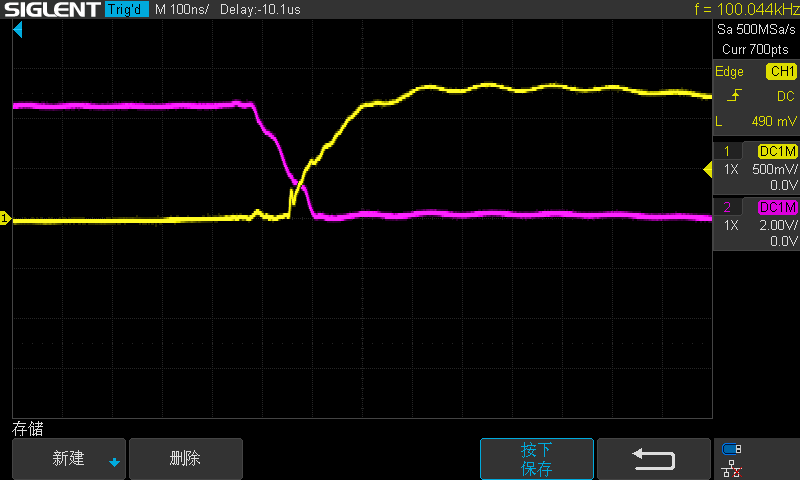
\includegraphics[width=0.88\textwidth]{images/软开关/软开关-开启.png}
  \caption{主开关 MOS 开通过程软开关波形}
  \label{fig:soft_switching_turn_on}
\end{figure}

\subsubsection{上位机与App功能测试}

上位机和 App 功能测试验证远程显示和参数交互。测试内容包括：

\begin{table}[htbp]
  \centering
  \caption{上位机与App功能测试结果}
  \label{tab:app_test}
  \begin{tabular}{@{}lp{5.5cm}@{}}
    \toprule
    \textbf{测试项目} & \textbf{结果} \\
    \midrule
    状态显示      & 电压、电流、SOC、温度实时刷新正常 \\
    模式控制      & 待机/运行/充电/放电命令可正确解析 \\
    参数交互      & 限值参数和查询命令响应正常 \\
    故障提示      & BMS 异常时界面正确显示告警 \\
    安全约束      & 禁止条件下拒绝充放电命令 \\
    \bottomrule
  \end{tabular}
\end{table}
\vspace{-0.3em}
{\small 资料来源：作者实测。}

% TODO: 替换为实际上位机/App/Web界面截图
\begin{figure}[htbp]
  \centering
  \fbox{\parbox[c][4cm][c]{0.88\linewidth}{\centering
  此处插入实际上位机/App/Web界面截图\\
  （显示电压/电流/SOC/温度/模式等实时数据）
  }}
  \caption{Web监控界面}
  \label{fig:app_screenshot}
\end{figure}

\subsubsection{模式切换与充放电测试}

系统支持待机、运行监控、充电、放电、降级和故障六种模式。模式切换测试验证主控状态机能否根据用户指令和 BMS 安全状态正确切换。关键测试结论：

\begin{itemize}[leftmargin=*,itemsep=0.3ex]
  \item 系统上电后正常进入待机模式，初始化完成后等待指令
  \item 用户下发运行命令且无严重故障时，正常进入运行监控模式
  \item BMS 允许充电且无故障时，可正确进入充电模式；BMS 禁止时拒绝切换
  \item BMS 允许放电且无故障时，可正确进入放电模式；BMS 禁止时拒绝切换
  \item 故障条件下系统进入降级或故障模式，FET 关断并上报告警
\end{itemize}

由于主功率级尚未完成额定工况闭环验证，本阶段充放电测试主要在低功率条件下验证模式逻辑、通信链路和保护响应。测试结果表明主控能够根据 BMS 状态正确判断充放电条件，上位机和 App 能够同步显示状态变化。

\subsection{本章小结}

本章对系统测试进行了详细分析。电压采样最大误差为 $+4\,\mathrm{mV}$，电流采样在 $5\,\mathrm{A}$ 以内误差控制在 $50\,\mathrm{mA}$ 以内，SOC 估算最大偏差约 $4.2\%$，均衡功能可将单体电压差从 $100\,\mathrm{mV}$ 降至 $20\,\mathrm{mV}$，CC/CV 充电切换正常，CAN 通信丢包率约 $0.067\%$。系统联调表明各模块数据交互正常，能够根据 BMS 安全状态正确切换工作模式。虽然主功率级仍需进一步完成实物闭环验证，但现有测试结果证明系统控制、监测、通信和保护平台具备继续开展整机联调的基础。
